
\chapter{Erreurs de mesures}
Un système de mesure n'est jamais parfait puisqu'il est en général plus ou moins sensible à l'environnement (température, pression, humidité...), et même les étalons servant à la calibration de l'instrument ne sont qu'une matérialisation imparfaite de la définition de l'unité qu'ils sont chargés représenter. Par conséquent, toute mesure est inéluctablement attachée d'erreurs.

De manière générale, le but de la mesure est d'évaluer la valeur numérique d'une observable physique. Ce que l'on obtient en pratique est une valeur donnée par l'instrument de mesure. Soit cette valeur correspond directement à la valeur de l'observable (p. ex.: pied-é-coulisse), soit il faut encore utiliser une courbe de calibration p.ex. thermomètre à thermocouple.

Quoi qu'il en soit, la valeur numérique fournie par le mesurage ne sera jamais - ou alors sinon par pur hasard - exactement égale à la vraie valeur numérique de l'observable, en raison des erreurs de mesure, toujours présentes, jamais nulles. Et naturellement, les erreurs de mesures ne sont jamais connues - sinon il suffirait de corriger la valeur mesurée, et nous obtiendrions la vraie valeur de l'observable !

Notre objectif, en tant qu'opérateur du mesurage, sera donc non seulement de fournir la valeur numérique mesurée, mais aussi de donner l'incertitude associée à cette mesure, incertitude estimée à partir de l'analyse statistique des erreurs de mesure. précisons:

\begin{description}
    \item[L'erreur de mesure] est l'écart entre la valeur numérique de la mesure et la valeur vraie du mesurande. Elle varie de manière aléatoire entre deux mesures du même mesurande.
    \item[L'incertitude] quant à elle est notre estimation de l'impact des erreurs sur la valeur annoncée de la mesure (en général la moyenne des mesures). L'incertitude est une valeur forcément positive, elle indique l'intervalle dans lequel on estime que se trouve la vraie valeur du mesurande.
\end{description}
En d'autres termes, les erreurs sont subies, tandis que les incertitudes sont estimées.

\subsubsection*{Mais pourquoi donner une incertitude ? et est-ce toujours nécessaire ?}

Tout va dépendre de l'application. Si vous allez commander des planches chez votre menuisier pour fabriquer une cage à lapins dans votre jardin, pas besoin d'indiquer de tolérance pour vos cotes. Par défaut, on sait bien que les planches seront coupées typiquement avec une précision de l'ordre du millimètre, ce qui suffit largement.

\textbf{En revanche}, lors d'un processus de fabrication industriel ou de la conception d'un prototype, il est évident que l'on spécifie toujours une tolérance pour les pièces fabriquées. De fait, lors de la \textbf{vérification} des pièces, afin de voir si les spécifications de tolérance sont respectées, il sera indispensable d'évaluer l'erreur probable commise sur la mesure, et il sera bien entendu absolument nécessaire que cette incertitude soit bien inférieure à la tolérance sur les pièces.

Admettons par exemple que la spécification du diamètre d'un axe usiné soit de 20 mm avec une tolérance de $\pm$ 0.005 mm soit $\pm$ 5 $\mu$m. Il est simplement complètement évident que l'incertitude de notre mesure devra être significativement inférieure à 5 $\mu$m (disons typiquement 0.5 $\mu$m), sinon notre mesure n'aura aucun intérêt. Et à plus forte raison, ne pas donner l'incertitude associée à la mesure enlève tout intérêt à cette dernière ! Comment en effet savoir si la tolérance est respectée si nous n'avons aucune idée de la précision de la mesure ? Si par exemple la mesure indique 20.01 mm, est-ce réellement 20.01 mm ou alors, en fait, 19.99 mm, mais avec une erreur de mesure de 0.02 mm ? Impossible ici de décider si la pièce est bonne ou non. En revanche, si on mesure 19.997 mm et que l'incertitude sur la mesure est de 0.0005 mm, alors on sait que la vraie valeur du mesurande sera dans l'intervalle 19.9965 à 19.9975 mm, ce qui est inclus dans la marge de tolérance de 19.995 à 20.005 mm, et conduira à l'acceptation de la pièce.

Autre exemple: si une théorie scientifique prédit un résultat, par exemple la masse du fameux boson de Higgs, il est clair que le laboratoire (ici le CERN) effectuant la vérification de cette prédiction théorique devra préciser l'incertitude associée à la mesure. Si la valeur prédite par la théorie est à l'intérieur de la marge d'erreur de la mesure, alors il y aura de bonnes chances que la théorie soit correcte. Dans le cas contraire, tout va dépendre de l'écart en prédiction théorique et mesure. Si l'écart est vraiment très grand, et la mesure très précise, alors il y a de fortes chances que la théorie soit fausse. Par contre, si l'écart est petit, il y a plus de chances que ce soit la précision de la mesure qui soit discutable. Quoi qu'il en soit, on comprend bien que sans indication de l'incertitude associée à la mesure, impossible de se prononcer sur quoi que ce soit.

\newpage

\subsubsection*{Intervalle et niveau de confiance}

Mais ce n'est pas tout. Il faut encore préciser quel est le niveau de confiance que l'on peut accorder à l'estimation de l'incertitude. En d'autres termes, avec quelle probabilité peut-on affirmer que la vraie valeur du mesurande se trouve en effet dans l'intervalle donné par l'incertitude, c.-à-d. dans l'intervalle?
\begin{center}
    [moyenne - incertitude] à [moyenne + incertitude] ?
\end{center}
Le niveau de confiance de l'incertitude se calcule à partir de la connaissance de la distribution de probabilité des erreurs, dont on discute au cours d'analyse de données. Il est égal à la probabilité que la valeur du mesurande soit dans l'intervalle ci-dessus, probabilité qui n'est rien d'autre que la somme (ou l'intégrale) de la distribution de probabilité des erreurs de mesures entre les bornes $\pm$incertitude.

Pour connaître le niveau de confiance, il faut donc connaitre la distribution de probabilité des erreurs de mesure, et pour connaitre celle-ci, il faut faire un grand nombre de mesures. De toute manière, toute mesure demande toujours l'acquisition d'un nombre significatif de mesures individuelles, de manière à pouvoir déterminer, justement, l'incertitude.

\begin{center}
    \fbox{
        \begin{minipage}{15.3cm}
            \begin{center}
                \textbf{Un résultat de mesure sera ainsi toujours annoncé de la manière suivante}:\\
                $\text{résultat}=\text{valeur numérique}\pm\text{incertitude}\ [\text{unité}]$ (é n \%)
            \end{center}
        \end{minipage}
    }
\end{center}
où n'est le niveau de confiance associé à l'intervalle d'incertitude (ou intervalle de confiance).


Dans ce chapitre, nous allons simplement nous concentrer sur les différents types d'erreurs pouvant se retrouver en pratique. L'estimation des incertitudes et niveau de confiance est traité dans l'autre partie de ce cours : \textit{l'analyse de données en sciences expérimentales}.

\newpage

\section{Causes probables des erreurs de mesure}

En toute généralité, les erreurs peuvent se classer en trois catégories :
\begin{description}
    \item[1) Les erreurs d'étalonnage]
    \item dues aux étalons primaires
    \item dues à la technique d'étalonnage
    \item[2) Les erreurs d'acquisition de données]
    \item dues aux capteurs
    \item dues à l'appareil de mesure
    \item dues aux variables non contrôlées
    \item[3) Les erreurs lors de l'analyse des données]
    \item dues au lissage (p.ex. méthode des moindres carrés)
    \item dues à la troncature (conversion analogique digitale)
\end{description}
On donne ci-après \textbf{quelques exemples} des causes d'erreur les plus fréquentes. La liste n'est pas exhaustive: seul un examen approfondi du processus de mesurage pour un instrument donné permettra de déterminer l'ensemble et l'origine des erreurs possibles.

\subsection{Erreurs d'étalonnage ou de calibration}

La grandeur étalon utilisée pour calibrer le système peut être elle-même entachée d'une petite erreur (différence entre la valeur réelle et la valeur annoncée). Par ailleurs, la mise en \oe uvre de la procédure d'étalonnage est elle aussi sujette à des erreurs, car la calibration est elle aussi une mesure ! Bien entendu, la calibration d'un instrument va se faire avec de grandes précautions, mais des erreurs seront toujours présentes: les erreurs d'étalonnage.

\subsection{Hystérésis}

Balayons la plage de valeurs d'entrée d'un système en partant de la plus petite valeur vers la plus grande puis de la plus grande vers la plus petite. En raison des frottements (pour un système mécanique), ou de la viscosité (système hydraulique) ou des charges électriques résiduelles (système électrique), la valeur finale sera légèrement différente de la valeur de départ. Pour une même valeur d'entrée, un système soumis à de l'hystérésis donnera par conséquent deux valeurs différentes suivant le sens de balayage. L'erreur d'hystérésis sur la mesure $M$ est alors définie par
$$
    \epsilon_h\ [\%]=100\,\left|\frac{M_{\text{max}}-M_{\text{min}}}{\text{moyenne}\{M\}}\right|
$$

\subsection{Erreur de linéarité}

La plupart des instruments sont connus pour fournir une relation linéaire entre la valeur physique entrée dans le système et la valeur de sortie. Mais comme les systèmes réels ne sont jamais parfaitement linéaires, une erreur est introduite à ce niveau, caractérisée par
$$
    \epsilon_\text{lin}\ [\%]=100\,\left|\frac{M-M_{\text{lin}}}{M}\right|
$$
où $M_{\text{lin}}$ est la valeur donnée par le système s'il était linéaire.

\subsection{Erreur de sensibilité}

Dans la situation où la mesure est réalisée à l'aide d'un capteur, il faut encore passer par la courbe de calibration de ce dernier pour déterminer la mesure dans l'unité qui nous intéresse (par exemple dans le cas du thermocouple la tension est transformée en une température). Si le système est linéaire, une erreur dans l'application du facteur de transformation (ou gain ou sensibilité), pour une raison quelconque (parce que le gain est mal connu, par exemple) engendre ce que l'on appelle l'erreur de sensibilité.

\subsection{Erreur due à la résolution de l'instrument}

L'erreur due à la résolution $\rho$ de l'instrument (voir le chapitre 3) peut être évaluée par
$$\epsilon_{\text{res}}=\pm\,\rho\,/\,2$$
car $\rho/2$ est l'écart maximal possible entre la valeur mesurée et la valeur affichée: la mesure sera toujours affichée à la valeur la plus proche possible que peut donner l'affichage.

\subsection{Grandeurs d'influence externes}

Le système peut, lors de son utilisation, être soumis en plus du mesurande à l'influence d'autres grandeurs physiques dont les variations peuvent modifier la valeur de la grandeur de sortie, et qui sont impossibles à distinguer de celle due à l'action du mesurande. Les principales grandeurs d'influence sont les suivantes (la liste n'est pas exhaustive) :
\begin{description}
    \item[la température,] qui a des effets électriques, mécaniques, géométriques (dilatation);
    \item[la pression,] qui a un effet mécanique;
    \item[l'accélération et les vibrations,] qui génèrent déformations et contraintes;
    \item[l'humidité,] qui a un effet sur les constantes diélectriques, la résistivité, l'isolation;
    \item[le champ électromagnétique,] qui génère une force électromotrice et agit sur la résistivité;
    \item[la tension d'alimentation de l'instrument,] qui peut varier en amplitude et en fréquence.
\end{description}
On cherchera à réduire au maximum non seulement l'amplitude, mais aussi et surtout la variation temporelle des grandeurs d'influence. En effet, si ces dernières sont stables, les erreurs engendrées seront constantes, donc systématiques, et il sera toujours possible de les identifier lors du processus de calibration: la courbe de calibration sera additionnée d'une valeur systématique non nulle même lorsque le mesurande est nul, représentant l'effet systématique des grandeurs d'influence, qu'il suffira de soustraire aux valeurs mesurées.

En revanche, si les grandeurs d'influence sont d'amplitude variable dans le temps, et de manière aléatoire et inconnue, alors il ne sera pas possible de s'affranchir de leur effet. Il conviendra alors de minimiser leur impact (par exemple, refroidissement stabilisé de l'appareil de mesure si la température est une grandeur d'influence critique).

\section{définitions de l'erreur et de l'incertitude}

\begin{wrapfigure}[10]{l}[6pt]{6cm}
    \centering
    \vspace{-5.5mm}
    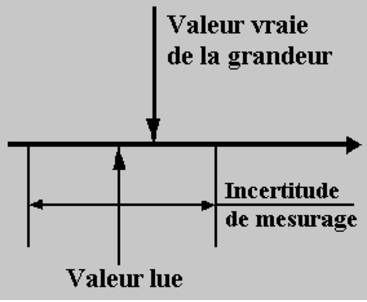
\includegraphics[width=6cm]{assets/figures/errinc.pdf}
\end{wrapfigure}

\textbf{L'erreur de mesure} est définie comme la différence entre la valeur annoncée et la valeur vraie qui reste inconnue. On ne connait jamais la valeur de l'erreur ni son signe, en revanche on peut estimer sa valeur absolue, en effectuant une calibration, et/ou un grand nombre de mesures.

\textbf{L'incertitude de mesure} décrit une région \textbf{autour} de la valeur mesurée dans laquelle on estime que se trouve la vraie valeur de l'observable. L'incertitude est un nombre que l'on calcule, à partir de la connaissance de la statistique des erreurs. Elle peut être annoncée de deux manières:
\begin{description}
    \item[absolue,] auquel cas elle a la même unité que la grandeur mesurée;
    \item[relative,] et se ramener à la valeur moyenne de l'observable, auquel cas elle est sans dimension et est généralement donnée en pourcentage \% de la valeur moyenne.
\end{description}

\begin{center}
    \fbox{\begin{minipage}{10cm}\textbf{Une mesure sans indication d'incertitude est une mesure pratiquement inutile. On s'attachera donc à déterminer l'incertitude avec le même soin que celui apporté à la mesure de la valeur elle-même.}\end{minipage}}
\end{center}

\begin{wrapfigure}[10]{l}[6pt]{7cm}
    \centering
    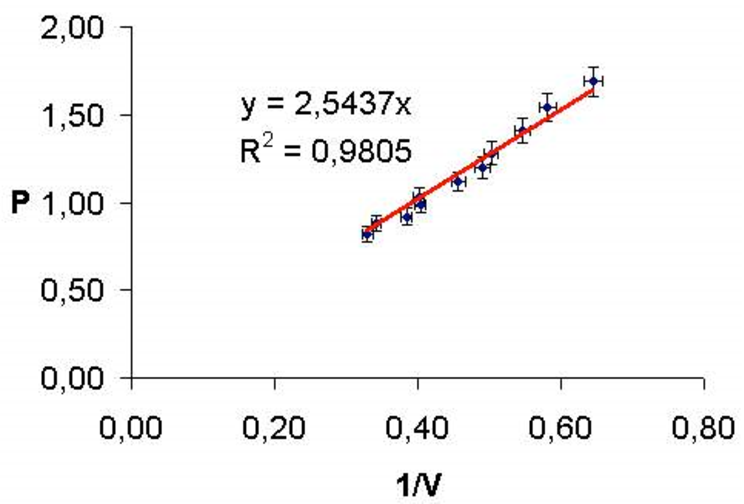
\includegraphics[width=7cm]{assets/figures/errbar.pdf}
    \caption{Graphique de données expérimentales avec barres d'erreur.}
    \label{fig:errbar}
\end{wrapfigure}
Sur un graphique de données expérimentales, l'incertitude de mesure sera décrite à l'aide de barres d'erreur, comme en figure \ref{fig:errbar}.

\section{Comment annoncer un résultat: les chiffres significatifs}

L'incertitude est une grandeur que l'opérateur du mesurage a la responsabilité d'estimer, afin d'être indiqué avec la valeur de la mesure. L'incertitude n'est cependant elle-même rien d'autre qu'une valeur approximative ! car il faudrait une infinité de mesures, et une connaissance absolue des caractéristiques de l'instrument de mesure pour pouvoir évaluer avec précision l'erreur probable commise de la mesure.

Par conséquent, lorsque l'on annonce la valeur de l'incertitude, il n'y a aucun sens à annoncer plus de 1 (voir 2) chiffre significatif. De même, il n'y a aucun sens à donner, dans la valeur annoncée du résultat de la mesure, des chiffres d'ordre décimal en dessous de la valeur de l'incertitude. Admettons par exemple que la valeur d'une mesure soit $V=9.876543$ et que l'incertitude estimée, dans la même unité, soit $E=0.004321$. On arrondira alors l'incertitude au premier chiffre significatif, soit $E=0.004$, et on arrondira la valeur $V$ à la décimale associée à $E$, soit à $10^{-3}$ ici. On énoncera alors le résultat de la manière suivante :
$$
    V=9.877\pm0.004\ \ \text{[unité]}
$$
Si cela est requis, il faudra encore donner le niveau de confiance de l'intervalle d'incertitude,
$$
    V=9.877\pm0.004\ \ \text{[unité], à 95 \%}
$$

\section{Erreurs systématiques et erreurs aléatoires}

\subsection{généralités}

L'incertitude comprend les effets d'erreurs \textbf{systématiques} et d'erreurs \textbf{aléatoires}, qui dépendent de la précision et résolution de l'instrument.

\textbf{L'erreur systématique} $\epsilon_s$ est la moyenne qui résulterait d'un nombre \textbf{infini} de mesurages du même mesurande, effectués dans des conditions de répétabilité, \textbf{moins} la valeur vraie du mesurande. En général, et à moins que l'instrument ne puisse être considéré d'une précision parfaite, l'erreur systématique et ses causes ne peuvent être connues qu'en partie. Les effets des erreurs systématiques, quand ils ne peuvent pas être corrigés, sont évalués d'après l'expérience acquise ou d'après d'autres informations.

\textbf{L'erreur aléatoire} $\epsilon_a$ est définie comme le résultat d'un \textbf{seul} mesurage moins la \textbf{moyenne} d'un nombre infini de mesurages, effectués dans des conditions de répétabilité absolue. Comme on ne peut faire qu'un nombre limité (fini) de mesurages, il n'est pas possible de déterminer avec une précision arbitrairement petite la moyenne des mesurages, et de fait, l'erreur aléatoire est elle-même sujette à une incertitude... L'amplitude des \textbf{erreurs aléatoires} peut cependant être évaluée à partir de la statistique des résultats de séries de mesurages (voir cours \textit{Analyse de données en sciences expérimentales}).

À ces deux erreurs peuvent s'ajouter les \textbf{erreurs grossières}, dues à des conditions anormales ou à des fautes techniques, et qui se manifesteront généralement par des valeurs mesurées considérablement différentes de toutes les autres valeurs.
\begin{figure}[t]
    \centering
    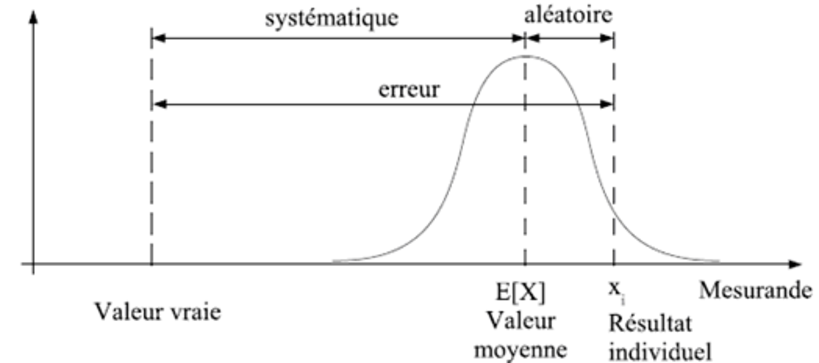
\includegraphics[width=14cm]{assets/figures/errsysale.pdf}
    \caption{Erreurs systématiques et aléatoires.}
    \label{fig:example}
\end{figure}

\subsection{Traitement des erreurs systématiques}

\subsubsection{Erreurs systématiques connues}

Les erreurs systématiques connues d'une mesure sont des grandeurs pouvant être déterminées tant du point de leur intensité que de leur signe. Les normes (ex. DIN1319) fournissent d'autres désignations telles que : erreurs systématiques avec signe connu, erreurs systématiques pures, erreurs corrigibles.

Un résultat peut être corrigé des erreurs systématiques connues. Lorsque la correction a été effectuée, les erreurs systématiques connues ne font plus partie de l'indication d'incertitude de mesure. Exemples d'erreurs systématiques connues:
\begin{itemize}

    \item Une cale-étalon plus longue de 0.7 $\mu$m que la valeur nominale indiquée;
    \item Une mesure de longueur effectuée à une température de 25$^{\circ}$C au lieu de la température de référence de 20$^{\circ}$C, produisant une erreur systématique à la suite de la dilatation thermique de l'objet;
    \item Un palmer qui possède des touches de palpage présentant une usure mesurable;
    \item Le tachymètre d'une voiture qui présente une indication de 5 km/h trop élevée dans une certaine plage;
    \item Un voltmètre dont on a vérifié qu'il possède un facteur d'amplification erroné ou indique une valeur trop élevée de 0.1 V dans toutes ses mesures.
\end{itemize}

\subsubsection{Erreurs systématiques inconnues}

Il existe aussi des erreurs systématiques inconnues qui sont généralement dues à des imprécisions des instruments : celles-ci sont normalement définies en termes de valeurs (ou tolérances) maximums, souvent avec le signe $\pm$. Il se peut que ces erreurs soient constantes dans une série de mesures avec un équipement particulier, mais on ne connaît \textit{ni} leur valeur \textit{ni} leur signe. On définit souvent les erreurs systématiques inconnues comme des \textbf{erreurs de tolérance}.

Les méthodes pour prendre en compte les erreurs systématiques inconnues dans un calcul global d'incertitude font l'objet d'études et de controverses depuis près de 200 ans, et le sujet reste controversé encore aujourd'hui.

Une approche fréquemment utilisée est la méthode \textit{ISO Guide to the Expression of Uncertainty in Measurement (GUM)}. L'idée de la méthode GUM est de " transformer " les erreurs systématiques inconnues en erreurs aléatoires, en postulant une distribution statistique ad hoc, généralement rectangulaire.

\subsection{Traitement des erreurs aléatoires}

On distingue en métrologie deux types d'erreurs aléatoires\footnote{La denomination type A ou B se référe au \textit{ISO Guide to the Expression of Uncertainty in Measurement} - la méthode GUM} :
\begin{description}
    \item[Type A] Les erreurs aléatoires dont la valeur peut être estimée par des méthodes statistiques;
    \item[Type B] Les erreurs systématiques inconnues " converties " en erreurs pseudo-aléatoires et qui demandent pour leur évaluation la prise en compte additionnelle d'aspects non statistiques tels que les caractéristiques et tolérances techniques de l'instrument, la précision et fiabilité de l'étalonnage, l'expérience de l'opérateur, etc..
\end{description}

\subsubsection{Erreurs aléatoires de type A - évaluées par des méthodes statistiques}

Ces erreurs aléatoires sont en général dues à des fluctuations des conditions environnementales (au sens large, ce qui inclut l'opérateur et l'instrument) au cours de la mesure. Ces erreurs sont par conséquent inconnues, tant du point de vue de leur intensité que de leur signe. Lors de mesures répétées au cours d'une série, on trouve que
\begin{enumerate}
    \item les  erreurs aléatoires fluctuent de manière imprévisible par rapport à une valeur moyenne;
    \item l'incertitude sur la moyenne diminue avec le nombre de mesures.
\end{enumerate}

On qualifie ces erreurs aléatoires, qui ont souvent une distribution normale\footnote{voir le cours " Analyse de données en sciences expérimentales "}, par leur écart-type.

Exemples d'erreurs aléatoires de type A :
\begin{itemize}

    \item Bruit d'instruments électroniques (amplificateurs) produisant des fluctuations du signal transmis.
    \item Influence de vibrations mécaniques sur l'instrument de mesure.
    \item Jeux des roulements ainsi que des flexions d'arbres de dispositifs mécaniques.
    \item Jeux d'articulations de palpeurs.
    \item Erreurs de lecture des graduations d'un microscope en raison d'une netteté insuffisante.
    \item Erreurs de positionnement d'un palpeur sur l'objet à mesurer au cours d'une série de mesures.
    \item Fluctuation de la température ambiante à la suite d'un défaut de régulation thermostatique ou par ouverture et fermeture répétée d'une porte du local de mesure. Une fluctuation de la température de l'objet à mesurer peut également intervenir à la suite d'un contact avec la main de l'opérateur.
    \item Influence de la fluctuation aléatoire du champ électrique et magnétique sur l'indicateur d'instruments de mesure électriques.
\end{itemize}

\subsubsection{Erreurs pseudo-aléatoires de type B - évaluées par des méthodes non statistiques}

Parmi de telles erreurs se trouvent, typiquement, les tolérances des instruments de mesure. Leur amplitude ainsi que leur signe au moment d'une mesure déterminée sont inconnus. Toutefois leur présence ainsi que l'intensité maximale (tolérance) est connue.

Dans le cadre de mesures répétées dans une série de mesures, il se peut que ces erreurs systématiques inconnues aient toujours la même valeur et le même signe.  Le problème est que cette valeur ainsi que ce signe sont inconnus : on ne connait en général que la valeur maximale.

Exemples d'erreurs de ce type:
\begin{itemize}

    \item La résolution d'un affichage numérique;
    \item Un palmer qui possède une tolérance connue de 0.3 $\mu$m. On ne sait cependant pas si l'erreur est de -0.3 $\mu$m ou +0.3 $\mu$m;
    \item Le cas oé, lors d'une mesure de longueur, la température de l'objet n'est pas mesurée. On sait cependant qu'au cours des mesures, la température se trouvait dans la tolérance de $\pm1^{\circ}$C par rapport à la température de référence de 20$^{\circ}$C;
    \item Une jauge qui possède une grandeur nominale de 30.000 mm et une indication de tolérance de $\pm 1\mu$m.
\end{itemize}
On remarquera que les erreurs de type B se distinguent des erreurs de type A par le fait qu'elles ne peuvent normalement pas être diminuées en augmentant le nombre de mesures effectuées.

Les erreurs de ce type peuvent être déterminées ou estimées de plusieurs manières, selon le cas:

À partir des caractéristiques de l'instrument donnés par le fabricant. Par exemple, si d'après ce dernier, la linéarité d'un voltmètre est de 0.1\% de la gamme de mesure de 300 V, il en résulte une erreur systématique inconnue de $\pm$0.3 V, à laquelle on associera une distribution rectangulaire \footnote{voir le cours " Analyse de données en sciences expérimentales "};
\begin{itemize}
    \item Comparaison avec un instrument de mesure au moins dix fois plus précis;
    \item Calcul des tolérances à partir des tolérances mécaniques et des relations géométriques de l'instrument de mesure, par exemple en cas de dilatation thermique.
\end{itemize}

\subsection{Traitement des erreurs grossières}

Après chaque série de mesures, il faut détecter et éliminer les erreurs grossières. L'origine de ces dernières doit aussitôt être élucidée de manière à ce que cette situation ne se reproduise plus au cours des séries de mesures suivantes. Si elles ne sont pas \textbf{éliminées} elles peuvent influencer considérablement la valeur moyenne et l'écart-type d'une série de mesures.

Quelques exemples d'erreurs grossières :
\begin{itemize}
    \item Les premières valeurs d'une série de mesures peuvent être erronées si l'appareil de mesure ne fournit des valeurs fiables qu'après un certain temps d'échauffement;
    \item Fausse lecture d'une mesure, par exemple par une erreur de virgule ou du facteur x10, x100 affiché;
    \item Les éléments d'une chaîne de mesure ne sont pas correctement adaptés en impédance;
    \item Tension d'alimentation fausse ou fluctuante;
    \item Choc contre l'instrument de mesure au cours du mesurage;
    \item L'appareil utilisé est défectueux en raison d'une chute antérieure;
    \item Mauvaise manipulation de l'appareil en raison de la méconnaissance du mode d'emploi de ce dernier.
\end{itemize}

%\end{document}
